% chapters/proposal-phase1.tex
% Replace the content below with your own text.

\section{Work Completed – Phase I: X-GAN}
\label{sec:xgan}
\subsection{Objective}

We developed a lightweight physics-informed denoising model for chest X-rays. The model has 2.17 million parameters. It balances noise suppression with the retention of fine anatomical features such as bone trabeculae and lung markings.
\subsection{Methodology}

Figure~\ref{fig:xgan_architecture} shows the architecture of X-GAN.

\begin{figure}[H]
	\centering
	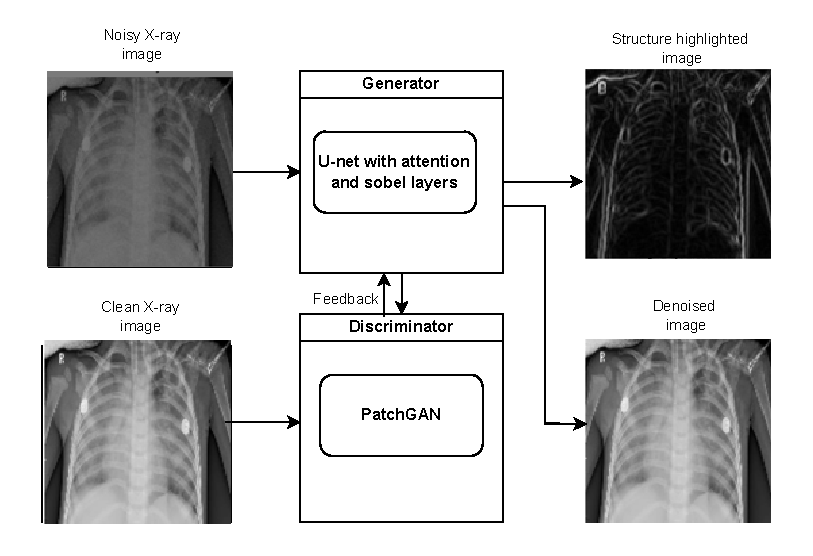
\includegraphics[width=0.85\textwidth]{images/XGAN-block.pdf}
	\caption{Architecture of X-GAN. The generator uses a U-Net with an edge attention mechanism at the bottleneck. The discriminator uses a PatchGAN with spectral normalisation.}
	\label{fig:xgan_architecture}
\end{figure}

The generator uses a U-Net architecture. We added an edge attention mechanism at the bottleneck layer. This mechanism computes gradient information using a Sobel operator and uses it to create spatial and channel-wise attention maps. The discriminator uses a PatchGAN architecture with spectral normalisation to stabilise training.

The loss function combines three components:

\[
L_{\text{total}} = \alpha L_{\text{MAE}} + \beta L_{\text{Edge}} + \gamma L_{\text{SSIM}}
\]

We performed a sensitivity analysis to find the optimal weights. The best performance occurred at \(\alpha = 1\), \(\beta = 5\), \(\gamma = 2\).

We trained and evaluated X-GAN on the Mendeley chest X-ray dataset \citep{sait2020curated}. This dataset contains 9,208 posterior-anterior chest X-ray images. We split the data into 80\% for training, 10\% for validation, and 10\% for testing. Since clean X-ray images are naturally noise-free, we simulated low-dose acquisitions by adding Poisson noise to the clean images. The noise level was controlled by a peak photon parameter set to \(\lambda = 1000\). All images were resized to \(256 \times 256\) pixels and normalised to the range \([0,1]\).

\subsection{Results}

Table~\ref{tab:xgan} compares X-GAN with state-of-the-art methods.

\begin{table}[H]
	\centering
	\caption{Performance comparison on chest X-ray denoising}
	\label{tab:xgan}
	\begin{tabular}{lcccc}
		\toprule
		Model & PSNR (dB) & SSIM & EPI & Parameters (M) \\
		\midrule
		RIDNet & 34.80 & 0.89 & 0.547 & 1.79 \\
		CBDNet & 34.44 & 0.89 & 0.561 & 4.57 \\
		X-ReCNN & 35.53 & 0.94 & 0.579 & 0.09 \\
		CGAN & 30.21 & 0.79 & 0.347 & 179.88 \\
		\textbf{X-GAN} & \textbf{36.48} & \textbf{0.95} & \textbf{0.721} & \textbf{2.17} \\
		\bottomrule
	\end{tabular}
\end{table}

X-GAN achieves the highest PSNR, SSIM, and EPI. It has 98\% fewer parameters than a standard CGAN.

\subsubsection{Ablation study}

We performed a component-wise ablation study to isolate the contribution of each design choice. Table~\ref{tab:xgan_ablation} shows the progressive improvement.

\begin{table}[H]
	\centering
	\caption{Component-wise ablation study}
	\label{tab:xgan_ablation}
	\begin{tabular}{lcccc}
		\toprule
		Configuration & PSNR & SSIM & E.RMSE & EPI \\
		\midrule
		U-Net + MAE & 33.20 & 0.92 & 0.12 & 0.35 \\
		+ Hybrid Loss & 35.70 & 0.94 & 0.09 & 0.47 \\
		+ Edge Attention & 35.84 & 0.94 & 0.06 & 0.62 \\
		+ \(4 \times 4\) Kernels & 36.48 & 0.95 & 0.05 & 0.71 \\
		\bottomrule
	\end{tabular}
\end{table}

The hybrid loss gave the largest improvement in PSNR (2.5 dB). Adding edge attention improved EPI from 0.47 to 0.62, confirming that the attention mechanism specifically helps preserve edges. The larger kernels provided a final boost in both PSNR and EPI.

\subsubsection{Downstream classification}

To evaluate clinical utility, we used X-GAN as a preprocessing step for a diagnostic classifier. Table~\ref{tab:xgan_downstream} shows the classification performance.

\begin{table}[H]
	\centering
	\caption{Impact of X-GAN denoising on downstream classification}
	\label{tab:xgan_downstream}
	\begin{tabular}{lccc}
		\toprule
		Model & Input & Accuracy & F1-score \\
		\midrule
		VGG-16 & Noisy & 69.75\% & 0.636 \\
		VGG-16 & X-GAN denoised & 80.00\% & 0.796 \\
		ResNet-50 & Noisy & 54.55\% & 0.568 \\
		ResNet-50 & X-GAN denoised & 79.52\% & 0.718 \\
		EfficientNetV2 & Noisy & 72.75\% & 0.707 \\
		EfficientNetV2 & X-GAN denoised & 87.00\% & 0.860 \\
		\bottomrule
	\end{tabular}
\end{table}

Denoising with X-GAN improved classification accuracy across all three architectures. ResNet-50 showed the largest gain, from 54.55\% to 79.52\%. EfficientNetV2 achieved the highest overall accuracy of 87.00\% on denoised images.

\subsubsection{Clinical evaluation}

We conducted a blinded mean opinion score (MOS) study with two experienced radiologists. They rated 50 randomly selected images on a 5-point scale across four dimensions: noise suppression, texture preservation, artifact freedom, and diagnostic confidence. Table~\ref{tab:xgan_mos} shows the results.

\begin{table}[H]
	\centering
	\small
	\caption{Blinded MOS from two radiologists. Values are mean ± standard deviation on a 5-point scale. Higher is better for all metrics.}
	\label{tab:xgan_mos}
	\begin{tabular}{lcccc}
		\toprule
		Model & Noise Suppression & Texture Preservation & Artifact Freedom & Diagnostic Conf. \\
		\midrule
		Noisy Input & 1.34 ± 0.51 & 4.92 ± 0.31 & 5.00 ± 0.00 & 2.20 ± 0.60 \\
		CBDNet & 4.04 ± 0.40 & 2.10 ± 0.50 & 4.02 ± 0.40 & 2.90 ± 0.50 \\
		RIDNet & 4.20 ± 0.49 & 2.98 ± 0.40 & 3.96 ± 0.40 & 3.30 ± 0.52 \\
		CGAN & 3.40 ± 0.71 & 3.00 ± 0.80 & 1.90 ± 0.59 & 2.40 ± 0.71 \\
		X-ReCNN & 4.90 ± 0.30 & 3.10 ± 0.50 & 4.60 ± 0.49 & 3.96 ± 0.40 \\
		\textbf{X-GAN} & \textbf{4.84 ± 0.36} & \textbf{4.70 ± 0.46} & \textbf{4.90 ± 0.30} & \textbf{4.90 ± 0.25} \\
		\bottomrule
	\end{tabular}
\end{table}

X-GAN achieved the highest diagnostic confidence score (4.90 ± 0.25), outperforming X-ReCNN (3.96 ± 0.40). It also scored highest in texture preservation (4.70 ± 0.46) and artifact freedom (4.90 ± 0.30). The noisy input scored low on noise suppression (1.34) but high on texture preservation (4.92) – this is expected because noise has not been removed. X-GAN successfully removes noise while keeping the natural texture intact.

\subsection{Conclusion of phase I}

X-GAN denoises chest X-rays while preserving edges. The hybrid loss function and edge attention mechanism work together to prevent over-smoothing. The ablation study confirms that each component contributes to the final performance. The downstream classification experiment shows that denoising improves diagnostic accuracy. The model has 2.17 million parameters, making it suitable for clinical deployment.
